%====================================================
\section{Lecture 2}

%====================================================
\subsection{Modulation}

In wireless communication, information cannot be transmitted efficiently at baseband over long distances. Antennas are physically inefficient at very low frequencies, and multiple users require frequency separation to share spectrum. 

To enable radiation and spectrum allocation, a baseband message signal $m(t)$ is shifted to a higher carrier frequency $f_c$. This process is called modulation.

The simplest modulation is:

\[
s(t) = m(t)\cos(2\pi f_c t).
\]

Here, $f_c$ determines where the signal appears in the spectrum. Modulation enables efficient transmission and multiplexing.

%====================================================
\subsection{Baseband and Bandpass Signals}

A baseband signal has spectrum centered at 0 Hz. Its bandwidth extends from $-B$ to $B$.

After modulation, the spectrum is shifted to $\pm f_c$, forming a bandpass signal.

Bandwidth is defined as:

\[
B = f_H - f_L.
\]

Spectral efficiency measures how efficiently bandwidth is used:

\[
\eta = \frac{R_b}{B}.
\]

%====================================================
\subsection{Amplitude Modulation (AM)}

In AM, the carrier amplitude varies with the message:

\[
s(t) = A_c [1 + k_a m(t)] \cos(2\pi f_c t).
\]

The modulation index is:

\[
\mu = k_a \max |m(t)|.
\]

If $\mu > 1$, overmodulation occurs and distortion appears.

AM is simple but inefficient in power because energy is transmitted in both the carrier and sidebands.

%====================================================
\subsection{Double Sideband Suppressed Carrier (DSB-SC)}

Removing the carrier produces:

\[
s(t) = m(t)\cos(2\pi f_c t).
\]

The bandwidth is:

\[
B_{DSB} = 2B.
\]

This improves power efficiency but still occupies twice the baseband bandwidth.

%====================================================
\subsection{Angle Modulation: FM and PM}

Frequency modulation (FM):

\[
s(t) = A_c \cos\left(2\pi f_c t + 2\pi k_f \int m(t) dt \right).
\]

Peak deviation:

\[
\Delta f = k_f A_m.
\]

Carson’s rule:

\[
B_{FM} = 2(\Delta f + B).
\]

Phase modulation (PM):

\[
s(t) = A_c \cos(2\pi f_c t + k_p m(t)).
\]

FM and PM are collectively called angle modulation and offer better noise immunity than AM.

%====================================================
\subsection{Complex Baseband Representation}

Bandpass signals can be expressed using complex notation:

\[
s(t) = I(t) + jQ(t) = A e^{j\theta}.
\]

Symbols are transmitted over finite time intervals:

\[
R_s = \frac{1}{T_s}.
\]

Bit rate:

\[
R_b = R_s \log_2 M.
\]

Increasing $M$ increases data rate but reduces noise tolerance.

%====================================================
\subsection{Electromagnetic Wave Propagation}

In free space, the electric field of a propagating wave is:

\[
E(f,t,r) = \frac{E_0}{r} e^{-j(2\pi f t - kr)},
\quad k = \frac{2\pi}{\lambda}.
\]

Amplitude decays as $\frac{1}{r}$ and power decays as $\frac{1}{r^2}$.

Free-space received power:

\[
P_r = P_t \left(\frac{\lambda}{4\pi d}\right)^2.
\]

Since $\lambda = \frac{c}{f_c}$, higher carrier frequencies suffer greater path loss.

More generally:

\[
PL(d) = PL(d_0) + 10n \log_{10}\left(\frac{d}{d_0}\right).
\]

%====================================================
\subsection{Multipath Propagation}

In realistic environments, signals reach the receiver via multiple paths due to reflection, diffraction, and scattering.

Each path has:
\[
\text{Amplitude } \alpha_i, \quad
\text{Delay } \tau_i, \quad
\text{Phase } \phi_i.
\]

Phase depends on distance:

\[
\phi = \frac{2\pi d}{\lambda}.
\]

Even small path differences create large phase shifts, producing constructive and destructive interference.

\begin{center}
\begin{tikzpicture}
\node (tx) at (0,0) {Tx};
\node (rx) at (8,0) {Rx};
\node (obs) at (4,2) {Obstacle};
\draw[->] (tx) -- (rx);
\draw[->] (tx) -- (obs);
\draw[->] (obs) -- (rx);
\draw[->] (tx) to[out=-40,in=-140] (rx);
\end{tikzpicture}
\end{center}

This causes fading and inter-symbol interference (ISI).

%====================================================
\subsection{Time Variation and Doppler}

Wireless channels vary over time due to motion and environmental changes.

Slow fading results from distance and shadowing.

Fast fading results from multipath interference.

Motion causes Doppler shift:

\[
f_D = \frac{v}{\lambda}\cos(\theta).
\]

Doppler introduces frequency spreading and limits coherence time.

%====================================================
\subsection{Linear Time-Varying Channel Model}

The wireless channel is modeled as:

\[
y(t) = \int h(t,\tau)x(t-\tau)d\tau + n(t).
\]

The impulse response is:

\[
h(t,\tau) = \sum_{i=1}^{N} \alpha_i(t)\delta(\tau - \tau_i).
\]

If only a Line-of-Sight (LOS) path exists:

\[
h(\tau) = \alpha_0 \delta(\tau - \tau_0),
\quad \tau_0 = \frac{D}{c}.
\]

%====================================================
\subsection{Power Delay Profile (PDP)}

The Power Delay Profile describes received power versus delay.

\begin{center}
\begin{tikzpicture}
\draw[->] (0,0) -- (8,0) node[right] {Delay};
\draw[->] (0,0) -- (0,3) node[above] {Power};
\draw[thick] (1,0) -- (1,2.5);
\draw[thick] (2.5,0) -- (2.5,1.8);
\draw[thick] (4,0) -- (4,1.2);
\draw[thick] (6,0) -- (6,0.6);
\end{tikzpicture}
\end{center}

Delay spread $T_d$ determines coherence bandwidth:

\[
W_c \approx \frac{1}{T_d}.
\]

If:

\[
B \ll W_c \Rightarrow \text{Flat fading}.
\]

If:

\[
B > W_c \Rightarrow \text{Frequency-selective fading}.
\]

%====================================================
\subsection{Four-Domain Channel Representation}

The wireless channel can be represented in four equivalent domains:

Time–Delay:
\[
h(t,\tau)
\]

Time–Frequency:
\[
H(f,t)
\]

Delay–Doppler:
\[
S(\tau,\nu)
\]

Frequency–Doppler:
\[
H(f,\nu)
\]

\begin{center}
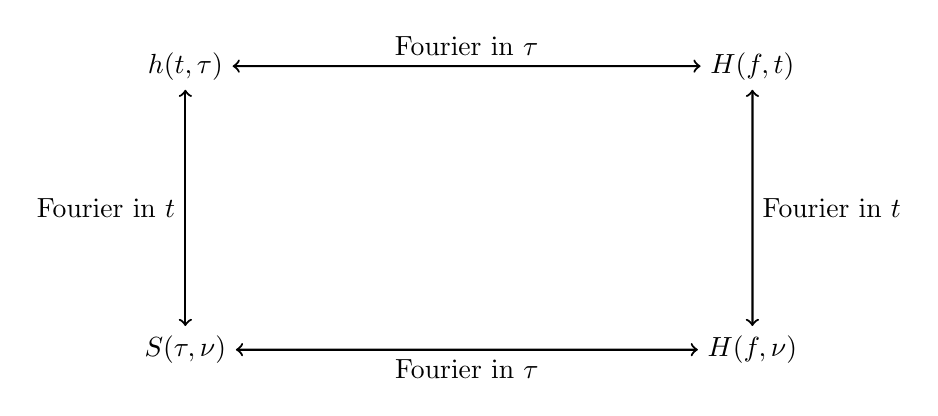
\begin{tikzpicture}[scale=1.2]
\node (ht) at (0,2) {$h(t,\tau)$};
\node (Hft) at (6,2) {$H(f,t)$};
\node (Stv) at (0,-1) {$S(\tau,\nu)$};
\node (Hfv) at (6,-1) {$H(f,\nu)$};
\draw[<->,thick] (ht) -- node[above]{Fourier in $\tau$} (Hft);
\draw[<->,thick] (Stv) -- node[below]{Fourier in $\tau$} (Hfv);
\draw[<->,thick] (ht) -- node[left]{Fourier in $t$} (Stv);
\draw[<->,thick] (Hft) -- node[right]{Fourier in $t$} (Hfv);
\end{tikzpicture}
\end{center}

Each representation emphasizes different physical aspects: delay spread, Doppler spread, frequency selectivity, and time variation.

%====================================================
\subsection{Noise and SNR}

Wireless systems are affected by Additive White Gaussian Noise (AWGN):

\[
y(t) = x(t) + n(t).
\]

Noise power over bandwidth $B$:

\[
P_n = N_0 B.
\]

Signal-to-noise ratio:

\[
\text{SNR} = \frac{P_s}{P_n}.
\]

%====================================================
\subsection{Multiple Access and Duplexing}

Spectrum is shared using:

FDMA (frequency separation),  
TDMA (time separation),  
CDMA (code separation),  
OFDM/OFDMA (subcarrier allocation).

Communication modes include simplex, half-duplex, and full-duplex.

%====================================================
